\documentclass[twoside]{book}

% Packages required by doxygen
\usepackage{calc}
\usepackage{doxygen}
\usepackage{graphicx}
\usepackage[utf8]{inputenc}
\usepackage{makeidx}
\usepackage{multicol}
\usepackage{multirow}
\usepackage{textcomp}
\usepackage[table]{xcolor}

% Font selection
\usepackage[T1]{fontenc}
\usepackage{mathptmx}
\usepackage[scaled=.90]{helvet}
\usepackage{courier}
\usepackage{amssymb}
\usepackage{sectsty}
\renewcommand{\familydefault}{\sfdefault}
\allsectionsfont{%
  \fontseries{bc}\selectfont%
  \color{darkgray}%
}
\renewcommand{\DoxyLabelFont}{%
  \fontseries{bc}\selectfont%
  \color{darkgray}%
}

% Page & text layout
\usepackage{geometry}
\geometry{%
  a4paper,%
  top=2.5cm,%
  bottom=2.5cm,%
  left=2.5cm,%
  right=2.5cm%
}
\tolerance=750
\hfuzz=15pt
\hbadness=750
\setlength{\emergencystretch}{15pt}
\setlength{\parindent}{0cm}
\setlength{\parskip}{0.2cm}
\makeatletter
\renewcommand{\paragraph}{%
  \@startsection{paragraph}{4}{0ex}{-1.0ex}{1.0ex}{%
    \normalfont\normalsize\bfseries\SS@parafont%
  }%
}
\renewcommand{\subparagraph}{%
  \@startsection{subparagraph}{5}{0ex}{-1.0ex}{1.0ex}{%
    \normalfont\normalsize\bfseries\SS@subparafont%
  }%
}
\makeatother

% Headers & footers
\usepackage{fancyhdr}
\pagestyle{fancyplain}
\fancyhead[LE]{\fancyplain{}{\bfseries\thepage}}
\fancyhead[CE]{\fancyplain{}{}}
\fancyhead[RE]{\fancyplain{}{\bfseries\leftmark}}
\fancyhead[LO]{\fancyplain{}{\bfseries\rightmark}}
\fancyhead[CO]{\fancyplain{}{}}
\fancyhead[RO]{\fancyplain{}{\bfseries\thepage}}
\fancyfoot[LE]{\fancyplain{}{}}
\fancyfoot[CE]{\fancyplain{}{}}
\fancyfoot[RE]{\fancyplain{}{\bfseries\scriptsize Generated on Fri May 5 2017 12\-:25\-:26 for T\-P\-\_\-\-M\-A\-L\-A\-F\-O\-S\-T\-\_\-\-M\-O\-R\-E\-L2 by Doxygen }}
\fancyfoot[LO]{\fancyplain{}{\bfseries\scriptsize Generated on Fri May 5 2017 12\-:25\-:26 for T\-P\-\_\-\-M\-A\-L\-A\-F\-O\-S\-T\-\_\-\-M\-O\-R\-E\-L2 by Doxygen }}
\fancyfoot[CO]{\fancyplain{}{}}
\fancyfoot[RO]{\fancyplain{}{}}
\renewcommand{\footrulewidth}{0.4pt}
\renewcommand{\chaptermark}[1]{%
  \markboth{#1}{}%
}
\renewcommand{\sectionmark}[1]{%
  \markright{\thesection\ #1}%
}

% Indices & bibliography
\usepackage{natbib}
\usepackage[titles]{tocloft}
\setcounter{tocdepth}{3}
\setcounter{secnumdepth}{5}
\makeindex

% Hyperlinks (required, but should be loaded last)
\usepackage{ifpdf}
\ifpdf
  \usepackage[pdftex,pagebackref=true]{hyperref}
\else
  \usepackage[ps2pdf,pagebackref=true]{hyperref}
\fi
\hypersetup{%
  colorlinks=true,%
  linkcolor=blue,%
  citecolor=blue,%
  unicode%
}

% Custom commands
\newcommand{\clearemptydoublepage}{%
  \newpage{\pagestyle{empty}\cleardoublepage}%
}


%===== C O N T E N T S =====

\begin{document}

% Titlepage & ToC
\hypersetup{pageanchor=false}
\pagenumbering{roman}
\begin{titlepage}
\vspace*{7cm}
\begin{center}%
{\Large T\-P\-\_\-\-M\-A\-L\-A\-F\-O\-S\-T\-\_\-\-M\-O\-R\-E\-L2 }\\
\vspace*{1cm}
{\large Generated by Doxygen 1.8.5}\\
\vspace*{0.5cm}
{\small Fri May 5 2017 12:25:26}\\
\end{center}
\end{titlepage}
\clearemptydoublepage
\tableofcontents
\clearemptydoublepage
\pagenumbering{arabic}
\hypersetup{pageanchor=true}

%--- Begin generated contents ---
\chapter{Hierarchical Index}
\section{Class Hierarchy}
This inheritance list is sorted roughly, but not completely, alphabetically\-:\begin{DoxyCompactList}
\item \contentsline{section}{Dvector}{\pageref{classDvector}}{}
\item \contentsline{section}{Generateur\-Nombre\-Aleatoire}{\pageref{classGenerateurNombreAleatoire}}{}
\begin{DoxyCompactList}
\item \contentsline{section}{Generateur\-Park\-Miller}{\pageref{classGenerateurParkMiller}}{}
\end{DoxyCompactList}
\item \contentsline{section}{Park\-Miller}{\pageref{classParkMiller}}{}
\end{DoxyCompactList}

\chapter{Class Index}
\section{Class List}
Here are the classes, structs, unions and interfaces with brief descriptions\-:\begin{DoxyCompactList}
\item\contentsline{section}{\hyperlink{classDvector}{Dvector} }{\pageref{classDvector}}{}
\item\contentsline{section}{\hyperlink{classGenerateurNombreAleatoire}{Generateur\-Nombre\-Aleatoire} }{\pageref{classGenerateurNombreAleatoire}}{}
\item\contentsline{section}{\hyperlink{classGenerateurParkMiller}{Generateur\-Park\-Miller} }{\pageref{classGenerateurParkMiller}}{}
\item\contentsline{section}{\hyperlink{classParkMiller}{Park\-Miller} }{\pageref{classParkMiller}}{}
\end{DoxyCompactList}

\chapter{File Index}
\section{File List}
Here is a list of all files with brief descriptions\-:\begin{DoxyCompactList}
\item\contentsline{section}{src/\hyperlink{Dvector_8cpp}{Dvector.\-cpp} }{\pageref{Dvector_8cpp}}{}
\item\contentsline{section}{src/\hyperlink{Dvector_8h}{Dvector.\-h} \\*Classe implémentant des tableaux dynamiques et les opérations allant avec }{\pageref{Dvector_8h}}{}
\item\contentsline{section}{src/\hyperlink{GenerateurNombreAleatoire_8cpp}{Generateur\-Nombre\-Aleatoire.\-cpp} }{\pageref{GenerateurNombreAleatoire_8cpp}}{}
\item\contentsline{section}{src/\hyperlink{GenerateurNombreAleatoire_8h}{Generateur\-Nombre\-Aleatoire.\-h} }{\pageref{GenerateurNombreAleatoire_8h}}{}
\item\contentsline{section}{src/\hyperlink{GenerateurParkMiller_8cpp}{Generateur\-Park\-Miller.\-cpp} }{\pageref{GenerateurParkMiller_8cpp}}{}
\item\contentsline{section}{src/\hyperlink{GenerateurParkMiller_8h}{Generateur\-Park\-Miller.\-h} }{\pageref{GenerateurParkMiller_8h}}{}
\item\contentsline{section}{src/\hyperlink{gentest_8cpp}{gentest.\-cpp} }{\pageref{gentest_8cpp}}{}
\item\contentsline{section}{src/\hyperlink{main_8cpp}{main.\-cpp} }{\pageref{main_8cpp}}{}
\item\contentsline{section}{src/\hyperlink{ParkMiller_8cpp}{Park\-Miller.\-cpp} }{\pageref{ParkMiller_8cpp}}{}
\item\contentsline{section}{src/\hyperlink{ParkMiller_8h}{Park\-Miller.\-h} }{\pageref{ParkMiller_8h}}{}
\end{DoxyCompactList}

\chapter{Class Documentation}
\hypertarget{classDvector}{\section{Dvector Class Reference}
\label{classDvector}\index{Dvector@{Dvector}}
}


{\ttfamily \#include $<$Dvector.\-h$>$}

\subsection*{Public Member Functions}
\begin{DoxyCompactItemize}
\item 
\hyperlink{classDvector_adf0f620df0feef3311f7d198e649a298}{Dvector} ()
\item 
int \hyperlink{classDvector_a964b4f5cc235ba6aaf9c5e437318be87}{size} ()
\item 
\hyperlink{classDvector_a6ca045c78602ab23be94e8701669a73f}{Dvector} (const \hyperlink{classDvector}{Dvector} \&V)
\item 
\hyperlink{classDvector_a5ad403c9d2c948d16a166af4e17ff34e}{Dvector} (int s, double p=0)
\item 
\hyperlink{classDvector_a75dc16ec331e444df83f54a9d313961a}{Dvector} (std\-::string \&)
\item 
void \hyperlink{classDvector_af66e4bdf60171463c01eea1039eecdb1}{display} (std\-::ostream \&str)
\item 
void \hyperlink{classDvector_a6fecdca0fbad7f928403597e322234b1}{fill\-Randomly} ()
\item 
\hyperlink{classDvector_a3156d0776c5da1a15685970200ec6b96}{$\sim$\-Dvector} ()
\item 
double \& \hyperlink{classDvector_a8c4063a0e38bec740498b132165e3ec8}{operator()} (const int \&i) const 
\item 
\hyperlink{classDvector}{Dvector} \hyperlink{classDvector_afca545bd8d0d6087863dabf7c1d73954}{operator+} (double o)
\item 
\hyperlink{classDvector}{Dvector} \hyperlink{classDvector_aab08102f4b4ffb7824ad8a90980e0eff}{operator-\/} (double o)
\item 
\hyperlink{classDvector}{Dvector} \hyperlink{classDvector_a5f346f4f33d53517f03fcbe97de08184}{operator$\ast$} (double o)
\item 
\hyperlink{classDvector}{Dvector} \hyperlink{classDvector_a60c543afd629b1759643ffe5e8d9a853}{operator/} (double o)
\item 
\hyperlink{classDvector}{Dvector} \hyperlink{classDvector_a402617afbca77199f537110a8efc0e10}{operator-\/} ()
\item 
\hyperlink{classDvector}{Dvector} \hyperlink{classDvector_ac9aed3cdd57a33e2a3fc6cc9da59bf10}{operator$>$$>$} (double o)
\item 
\hyperlink{classDvector}{Dvector} \hyperlink{classDvector_a0642720ca4ecae9d6fe8cf24cf9cffd6}{operator$<$$<$} (double o)
\item 
\hyperlink{classDvector}{Dvector} \hyperlink{classDvector_a47c89af4906459043b66b5aba4b9cef4}{operator+=} (double o)
\item 
\hyperlink{classDvector}{Dvector} \hyperlink{classDvector_a1b3d3ea283f2ebb3b0566220df97c1fd}{operator-\/=} (double o)
\item 
\hyperlink{classDvector}{Dvector} \hyperlink{classDvector_a8cb4e4ffcb838428b0e22e982edb132f}{operator$\ast$=} (double o)
\item 
\hyperlink{classDvector}{Dvector} \hyperlink{classDvector_a06ef842c794c08c19525dd1065f8e739}{operator/=} (double o)
\item 
\hyperlink{classDvector}{Dvector} \hyperlink{classDvector_abf0bed6290ef45d7811b69732ad4a8cf}{operator=} (const \hyperlink{classDvector}{Dvector} \&V)
\item 
\hyperlink{classDvector}{Dvector} \hyperlink{classDvector_a3242a315e31b62886285e5d92af43a6f}{resize} (int \hyperlink{classDvector_a728a936adcb2a17365255656c5f94692}{taille}, double valeur=0.)
\end{DoxyCompactItemize}
\subsection*{Public Attributes}
\begin{DoxyCompactItemize}
\item 
int \hyperlink{classDvector_a728a936adcb2a17365255656c5f94692}{taille}
\end{DoxyCompactItemize}
\subsection*{Friends}
\begin{DoxyCompactItemize}
\item 
\hyperlink{classDvector}{Dvector} \hyperlink{classDvector_adc04cf82aee079aca57cf20806737afe}{operator+} (const \hyperlink{classDvector}{Dvector} \&n, const \hyperlink{classDvector}{Dvector} \&v)
\item 
\hyperlink{classDvector}{Dvector} \hyperlink{classDvector_a73a2612ede73afd8f5e94fa2ae0d6aa4}{operator-\/} (const \hyperlink{classDvector}{Dvector} \&n, const \hyperlink{classDvector}{Dvector} \&v)
\item 
bool \hyperlink{classDvector_a78765ce7576547b645ccc54e0b22e7bf}{operator==} (const \hyperlink{classDvector}{Dvector} \&n, const \hyperlink{classDvector}{Dvector} \&v)
\end{DoxyCompactItemize}


\subsection{Constructor \& Destructor Documentation}
\hypertarget{classDvector_adf0f620df0feef3311f7d198e649a298}{\index{Dvector@{Dvector}!Dvector@{Dvector}}
\index{Dvector@{Dvector}!Dvector@{Dvector}}
\subsubsection[{Dvector}]{\setlength{\rightskip}{0pt plus 5cm}Dvector\-::\-Dvector (
\begin{DoxyParamCaption}
{}
\end{DoxyParamCaption}
)}}\label{classDvector_adf0f620df0feef3311f7d198e649a298}
\hypertarget{classDvector_a6ca045c78602ab23be94e8701669a73f}{\index{Dvector@{Dvector}!Dvector@{Dvector}}
\index{Dvector@{Dvector}!Dvector@{Dvector}}
\subsubsection[{Dvector}]{\setlength{\rightskip}{0pt plus 5cm}Dvector\-::\-Dvector (
\begin{DoxyParamCaption}
\item[{const {\bf Dvector} \&}]{V}
\end{DoxyParamCaption}
)}}\label{classDvector_a6ca045c78602ab23be94e8701669a73f}
\hypertarget{classDvector_a5ad403c9d2c948d16a166af4e17ff34e}{\index{Dvector@{Dvector}!Dvector@{Dvector}}
\index{Dvector@{Dvector}!Dvector@{Dvector}}
\subsubsection[{Dvector}]{\setlength{\rightskip}{0pt plus 5cm}Dvector\-::\-Dvector (
\begin{DoxyParamCaption}
\item[{int}]{s, }
\item[{double}]{p = {\ttfamily 0}}
\end{DoxyParamCaption}
)}}\label{classDvector_a5ad403c9d2c948d16a166af4e17ff34e}
\hypertarget{classDvector_a75dc16ec331e444df83f54a9d313961a}{\index{Dvector@{Dvector}!Dvector@{Dvector}}
\index{Dvector@{Dvector}!Dvector@{Dvector}}
\subsubsection[{Dvector}]{\setlength{\rightskip}{0pt plus 5cm}Dvector\-::\-Dvector (
\begin{DoxyParamCaption}
\item[{std\-::string \&}]{my\-\_\-str}
\end{DoxyParamCaption}
)}}\label{classDvector_a75dc16ec331e444df83f54a9d313961a}
\hypertarget{classDvector_a3156d0776c5da1a15685970200ec6b96}{\index{Dvector@{Dvector}!$\sim$\-Dvector@{$\sim$\-Dvector}}
\index{$\sim$\-Dvector@{$\sim$\-Dvector}!Dvector@{Dvector}}
\subsubsection[{$\sim$\-Dvector}]{\setlength{\rightskip}{0pt plus 5cm}Dvector\-::$\sim$\-Dvector (
\begin{DoxyParamCaption}
{}
\end{DoxyParamCaption}
)}}\label{classDvector_a3156d0776c5da1a15685970200ec6b96}


\subsection{Member Function Documentation}
\hypertarget{classDvector_af66e4bdf60171463c01eea1039eecdb1}{\index{Dvector@{Dvector}!display@{display}}
\index{display@{display}!Dvector@{Dvector}}
\subsubsection[{display}]{\setlength{\rightskip}{0pt plus 5cm}void Dvector\-::display (
\begin{DoxyParamCaption}
\item[{std\-::ostream \&}]{str}
\end{DoxyParamCaption}
)}}\label{classDvector_af66e4bdf60171463c01eea1039eecdb1}
\hypertarget{classDvector_a6fecdca0fbad7f928403597e322234b1}{\index{Dvector@{Dvector}!fill\-Randomly@{fill\-Randomly}}
\index{fill\-Randomly@{fill\-Randomly}!Dvector@{Dvector}}
\subsubsection[{fill\-Randomly}]{\setlength{\rightskip}{0pt plus 5cm}void Dvector\-::fill\-Randomly (
\begin{DoxyParamCaption}
{}
\end{DoxyParamCaption}
)}}\label{classDvector_a6fecdca0fbad7f928403597e322234b1}
\hypertarget{classDvector_a8c4063a0e38bec740498b132165e3ec8}{\index{Dvector@{Dvector}!operator()@{operator()}}
\index{operator()@{operator()}!Dvector@{Dvector}}
\subsubsection[{operator()}]{\setlength{\rightskip}{0pt plus 5cm}double \& Dvector\-::operator() (
\begin{DoxyParamCaption}
\item[{const int \&}]{i}
\end{DoxyParamCaption}
) const}}\label{classDvector_a8c4063a0e38bec740498b132165e3ec8}
\hypertarget{classDvector_a5f346f4f33d53517f03fcbe97de08184}{\index{Dvector@{Dvector}!operator$\ast$@{operator$\ast$}}
\index{operator$\ast$@{operator$\ast$}!Dvector@{Dvector}}
\subsubsection[{operator$\ast$}]{\setlength{\rightskip}{0pt plus 5cm}{\bf Dvector} Dvector\-::operator$\ast$ (
\begin{DoxyParamCaption}
\item[{double}]{o}
\end{DoxyParamCaption}
)}}\label{classDvector_a5f346f4f33d53517f03fcbe97de08184}
\hypertarget{classDvector_a8cb4e4ffcb838428b0e22e982edb132f}{\index{Dvector@{Dvector}!operator$\ast$=@{operator$\ast$=}}
\index{operator$\ast$=@{operator$\ast$=}!Dvector@{Dvector}}
\subsubsection[{operator$\ast$=}]{\setlength{\rightskip}{0pt plus 5cm}{\bf Dvector} Dvector\-::operator$\ast$= (
\begin{DoxyParamCaption}
\item[{double}]{o}
\end{DoxyParamCaption}
)}}\label{classDvector_a8cb4e4ffcb838428b0e22e982edb132f}
\hypertarget{classDvector_afca545bd8d0d6087863dabf7c1d73954}{\index{Dvector@{Dvector}!operator+@{operator+}}
\index{operator+@{operator+}!Dvector@{Dvector}}
\subsubsection[{operator+}]{\setlength{\rightskip}{0pt plus 5cm}{\bf Dvector} Dvector\-::operator+ (
\begin{DoxyParamCaption}
\item[{double}]{o}
\end{DoxyParamCaption}
)}}\label{classDvector_afca545bd8d0d6087863dabf7c1d73954}
\hypertarget{classDvector_a47c89af4906459043b66b5aba4b9cef4}{\index{Dvector@{Dvector}!operator+=@{operator+=}}
\index{operator+=@{operator+=}!Dvector@{Dvector}}
\subsubsection[{operator+=}]{\setlength{\rightskip}{0pt plus 5cm}{\bf Dvector} Dvector\-::operator+= (
\begin{DoxyParamCaption}
\item[{double}]{o}
\end{DoxyParamCaption}
)}}\label{classDvector_a47c89af4906459043b66b5aba4b9cef4}
\hypertarget{classDvector_aab08102f4b4ffb7824ad8a90980e0eff}{\index{Dvector@{Dvector}!operator-\/@{operator-\/}}
\index{operator-\/@{operator-\/}!Dvector@{Dvector}}
\subsubsection[{operator-\/}]{\setlength{\rightskip}{0pt plus 5cm}{\bf Dvector} Dvector\-::operator-\/ (
\begin{DoxyParamCaption}
\item[{double}]{o}
\end{DoxyParamCaption}
)}}\label{classDvector_aab08102f4b4ffb7824ad8a90980e0eff}
\hypertarget{classDvector_a402617afbca77199f537110a8efc0e10}{\index{Dvector@{Dvector}!operator-\/@{operator-\/}}
\index{operator-\/@{operator-\/}!Dvector@{Dvector}}
\subsubsection[{operator-\/}]{\setlength{\rightskip}{0pt plus 5cm}{\bf Dvector} Dvector\-::operator-\/ (
\begin{DoxyParamCaption}
{}
\end{DoxyParamCaption}
)}}\label{classDvector_a402617afbca77199f537110a8efc0e10}
\hypertarget{classDvector_a1b3d3ea283f2ebb3b0566220df97c1fd}{\index{Dvector@{Dvector}!operator-\/=@{operator-\/=}}
\index{operator-\/=@{operator-\/=}!Dvector@{Dvector}}
\subsubsection[{operator-\/=}]{\setlength{\rightskip}{0pt plus 5cm}{\bf Dvector} Dvector\-::operator-\/= (
\begin{DoxyParamCaption}
\item[{double}]{o}
\end{DoxyParamCaption}
)}}\label{classDvector_a1b3d3ea283f2ebb3b0566220df97c1fd}
\hypertarget{classDvector_a60c543afd629b1759643ffe5e8d9a853}{\index{Dvector@{Dvector}!operator/@{operator/}}
\index{operator/@{operator/}!Dvector@{Dvector}}
\subsubsection[{operator/}]{\setlength{\rightskip}{0pt plus 5cm}{\bf Dvector} Dvector\-::operator/ (
\begin{DoxyParamCaption}
\item[{double}]{o}
\end{DoxyParamCaption}
)}}\label{classDvector_a60c543afd629b1759643ffe5e8d9a853}
\hypertarget{classDvector_a06ef842c794c08c19525dd1065f8e739}{\index{Dvector@{Dvector}!operator/=@{operator/=}}
\index{operator/=@{operator/=}!Dvector@{Dvector}}
\subsubsection[{operator/=}]{\setlength{\rightskip}{0pt plus 5cm}{\bf Dvector} Dvector\-::operator/= (
\begin{DoxyParamCaption}
\item[{double}]{o}
\end{DoxyParamCaption}
)}}\label{classDvector_a06ef842c794c08c19525dd1065f8e739}
\hypertarget{classDvector_a0642720ca4ecae9d6fe8cf24cf9cffd6}{\index{Dvector@{Dvector}!operator$<$$<$@{operator$<$$<$}}
\index{operator$<$$<$@{operator$<$$<$}!Dvector@{Dvector}}
\subsubsection[{operator$<$$<$}]{\setlength{\rightskip}{0pt plus 5cm}{\bf Dvector} Dvector\-::operator$<$$<$ (
\begin{DoxyParamCaption}
\item[{double}]{o}
\end{DoxyParamCaption}
)}}\label{classDvector_a0642720ca4ecae9d6fe8cf24cf9cffd6}
\hypertarget{classDvector_abf0bed6290ef45d7811b69732ad4a8cf}{\index{Dvector@{Dvector}!operator=@{operator=}}
\index{operator=@{operator=}!Dvector@{Dvector}}
\subsubsection[{operator=}]{\setlength{\rightskip}{0pt plus 5cm}{\bf Dvector} Dvector\-::operator= (
\begin{DoxyParamCaption}
\item[{const {\bf Dvector} \&}]{V}
\end{DoxyParamCaption}
)}}\label{classDvector_abf0bed6290ef45d7811b69732ad4a8cf}
\hypertarget{classDvector_ac9aed3cdd57a33e2a3fc6cc9da59bf10}{\index{Dvector@{Dvector}!operator$>$$>$@{operator$>$$>$}}
\index{operator$>$$>$@{operator$>$$>$}!Dvector@{Dvector}}
\subsubsection[{operator$>$$>$}]{\setlength{\rightskip}{0pt plus 5cm}{\bf Dvector} Dvector\-::operator$>$$>$ (
\begin{DoxyParamCaption}
\item[{double}]{o}
\end{DoxyParamCaption}
)}}\label{classDvector_ac9aed3cdd57a33e2a3fc6cc9da59bf10}
\hypertarget{classDvector_a3242a315e31b62886285e5d92af43a6f}{\index{Dvector@{Dvector}!resize@{resize}}
\index{resize@{resize}!Dvector@{Dvector}}
\subsubsection[{resize}]{\setlength{\rightskip}{0pt plus 5cm}{\bf Dvector} Dvector\-::resize (
\begin{DoxyParamCaption}
\item[{int}]{taille, }
\item[{double}]{valeur = {\ttfamily 0.}}
\end{DoxyParamCaption}
)}}\label{classDvector_a3242a315e31b62886285e5d92af43a6f}
\hypertarget{classDvector_a964b4f5cc235ba6aaf9c5e437318be87}{\index{Dvector@{Dvector}!size@{size}}
\index{size@{size}!Dvector@{Dvector}}
\subsubsection[{size}]{\setlength{\rightskip}{0pt plus 5cm}int Dvector\-::size (
\begin{DoxyParamCaption}
{}
\end{DoxyParamCaption}
)}}\label{classDvector_a964b4f5cc235ba6aaf9c5e437318be87}


\subsection{Friends And Related Function Documentation}
\hypertarget{classDvector_adc04cf82aee079aca57cf20806737afe}{\index{Dvector@{Dvector}!operator+@{operator+}}
\index{operator+@{operator+}!Dvector@{Dvector}}
\subsubsection[{operator+}]{\setlength{\rightskip}{0pt plus 5cm}{\bf Dvector} operator+ (
\begin{DoxyParamCaption}
\item[{const {\bf Dvector} \&}]{n, }
\item[{const {\bf Dvector} \&}]{v}
\end{DoxyParamCaption}
)\hspace{0.3cm}{\ttfamily [friend]}}}\label{classDvector_adc04cf82aee079aca57cf20806737afe}
\hypertarget{classDvector_a73a2612ede73afd8f5e94fa2ae0d6aa4}{\index{Dvector@{Dvector}!operator-\/@{operator-\/}}
\index{operator-\/@{operator-\/}!Dvector@{Dvector}}
\subsubsection[{operator-\/}]{\setlength{\rightskip}{0pt plus 5cm}{\bf Dvector} operator-\/ (
\begin{DoxyParamCaption}
\item[{const {\bf Dvector} \&}]{n, }
\item[{const {\bf Dvector} \&}]{v}
\end{DoxyParamCaption}
)\hspace{0.3cm}{\ttfamily [friend]}}}\label{classDvector_a73a2612ede73afd8f5e94fa2ae0d6aa4}
\hypertarget{classDvector_a78765ce7576547b645ccc54e0b22e7bf}{\index{Dvector@{Dvector}!operator==@{operator==}}
\index{operator==@{operator==}!Dvector@{Dvector}}
\subsubsection[{operator==}]{\setlength{\rightskip}{0pt plus 5cm}bool operator== (
\begin{DoxyParamCaption}
\item[{const {\bf Dvector} \&}]{n, }
\item[{const {\bf Dvector} \&}]{v}
\end{DoxyParamCaption}
)\hspace{0.3cm}{\ttfamily [friend]}}}\label{classDvector_a78765ce7576547b645ccc54e0b22e7bf}


\subsection{Member Data Documentation}
\hypertarget{classDvector_a728a936adcb2a17365255656c5f94692}{\index{Dvector@{Dvector}!taille@{taille}}
\index{taille@{taille}!Dvector@{Dvector}}
\subsubsection[{taille}]{\setlength{\rightskip}{0pt plus 5cm}int Dvector\-::taille}}\label{classDvector_a728a936adcb2a17365255656c5f94692}


The documentation for this class was generated from the following files\-:\begin{DoxyCompactItemize}
\item 
src/\hyperlink{Dvector_8h}{Dvector.\-h}\item 
src/\hyperlink{Dvector_8cpp}{Dvector.\-cpp}\end{DoxyCompactItemize}

\hypertarget{classGenerateurNombreAleatoire}{\section{Generateur\-Nombre\-Aleatoire Class Reference}
\label{classGenerateurNombreAleatoire}\index{Generateur\-Nombre\-Aleatoire@{Generateur\-Nombre\-Aleatoire}}
}


{\ttfamily \#include $<$Generateur\-Nombre\-Aleatoire.\-h$>$}

Inheritance diagram for Generateur\-Nombre\-Aleatoire\-:\begin{figure}[H]
\begin{center}
\leavevmode
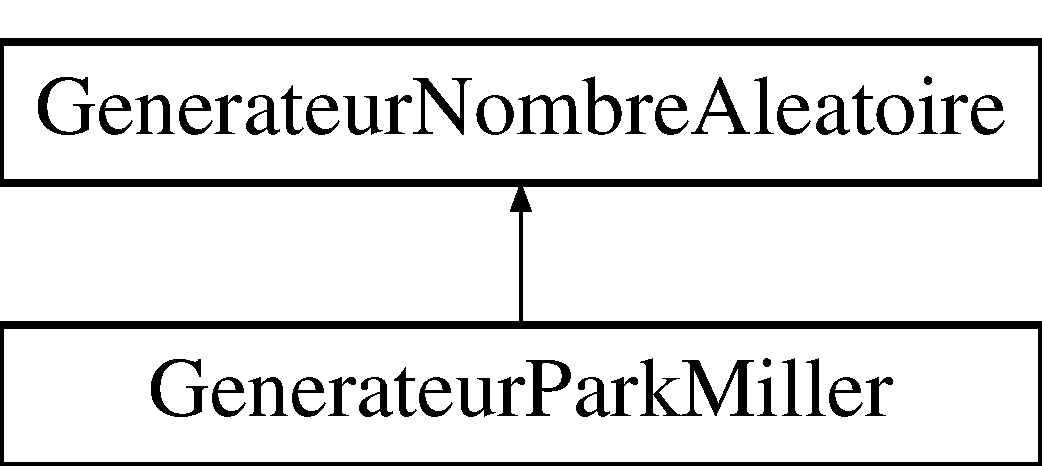
\includegraphics[height=2.000000cm]{classGenerateurNombreAleatoire}
\end{center}
\end{figure}
\subsection*{Public Member Functions}
\begin{DoxyCompactItemize}
\item 
\hyperlink{classGenerateurNombreAleatoire_ad6a159bdea95f54c4363b59944e80030}{Generateur\-Nombre\-Aleatoire} ()
\item 
\hyperlink{classGenerateurNombreAleatoire_aa39e185dcbd1356b28227b2ea24d8138}{Generateur\-Nombre\-Aleatoire} (int dim)
\item 
\hyperlink{classGenerateurNombreAleatoire_ad9a7dedf1f5f2ce3c3c3121f66e0fbed}{Generateur\-Nombre\-Aleatoire} (const \hyperlink{classGenerateurNombreAleatoire}{Generateur\-Nombre\-Aleatoire} \&Gen)
\item 
\hyperlink{classGenerateurNombreAleatoire}{Generateur\-Nombre\-Aleatoire} $\ast$ \hyperlink{classGenerateurNombreAleatoire_a93af1b3a6b970d2d5e5a078c22fa5478}{Clone} ()
\item 
\hyperlink{classGenerateurNombreAleatoire_a4b0f91e7003697042cc1d58f6f7fc313}{$\sim$\-Generateur\-Nombre\-Aleatoire} ()
\item 
\hyperlink{classGenerateurNombreAleatoire}{Generateur\-Nombre\-Aleatoire} \hyperlink{classGenerateurNombreAleatoire_a3f058a96aa678a3efb841c5ae5313917}{operator=} (const \hyperlink{classGenerateurNombreAleatoire}{Generateur\-Nombre\-Aleatoire} \&Gen)
\item 
int \hyperlink{classGenerateurNombreAleatoire_a378a808ce192f8e6e79197344b0adc95}{get\-Dim} ()
\item 
void \hyperlink{classGenerateurNombreAleatoire_ad189d10901dea1aea438a0fb10f65f47}{set\-\_\-seed} ()
\item 
int \hyperlink{classGenerateurNombreAleatoire_a2cd3efb7eedf9ab71084f77c9e02562d}{get\-\_\-seed} ()
\item 
void \hyperlink{classGenerateurNombreAleatoire_a40f479064b1d228de24e06bbb14969f6}{reset\-\_\-seed} ()
\item 
\hyperlink{classDvector}{Dvector} \hyperlink{classGenerateurNombreAleatoire_a8ae22e6422271e438df2089c4bc6a8b9}{gen\-Uniforme} ()
\end{DoxyCompactItemize}


\subsection{Constructor \& Destructor Documentation}
\hypertarget{classGenerateurNombreAleatoire_ad6a159bdea95f54c4363b59944e80030}{\index{Generateur\-Nombre\-Aleatoire@{Generateur\-Nombre\-Aleatoire}!Generateur\-Nombre\-Aleatoire@{Generateur\-Nombre\-Aleatoire}}
\index{Generateur\-Nombre\-Aleatoire@{Generateur\-Nombre\-Aleatoire}!GenerateurNombreAleatoire@{Generateur\-Nombre\-Aleatoire}}
\subsubsection[{Generateur\-Nombre\-Aleatoire}]{\setlength{\rightskip}{0pt plus 5cm}Generateur\-Nombre\-Aleatoire\-::\-Generateur\-Nombre\-Aleatoire (
\begin{DoxyParamCaption}
{}
\end{DoxyParamCaption}
)}}\label{classGenerateurNombreAleatoire_ad6a159bdea95f54c4363b59944e80030}
\hypertarget{classGenerateurNombreAleatoire_aa39e185dcbd1356b28227b2ea24d8138}{\index{Generateur\-Nombre\-Aleatoire@{Generateur\-Nombre\-Aleatoire}!Generateur\-Nombre\-Aleatoire@{Generateur\-Nombre\-Aleatoire}}
\index{Generateur\-Nombre\-Aleatoire@{Generateur\-Nombre\-Aleatoire}!GenerateurNombreAleatoire@{Generateur\-Nombre\-Aleatoire}}
\subsubsection[{Generateur\-Nombre\-Aleatoire}]{\setlength{\rightskip}{0pt plus 5cm}Generateur\-Nombre\-Aleatoire\-::\-Generateur\-Nombre\-Aleatoire (
\begin{DoxyParamCaption}
\item[{int}]{dim}
\end{DoxyParamCaption}
)}}\label{classGenerateurNombreAleatoire_aa39e185dcbd1356b28227b2ea24d8138}
\hypertarget{classGenerateurNombreAleatoire_ad9a7dedf1f5f2ce3c3c3121f66e0fbed}{\index{Generateur\-Nombre\-Aleatoire@{Generateur\-Nombre\-Aleatoire}!Generateur\-Nombre\-Aleatoire@{Generateur\-Nombre\-Aleatoire}}
\index{Generateur\-Nombre\-Aleatoire@{Generateur\-Nombre\-Aleatoire}!GenerateurNombreAleatoire@{Generateur\-Nombre\-Aleatoire}}
\subsubsection[{Generateur\-Nombre\-Aleatoire}]{\setlength{\rightskip}{0pt plus 5cm}Generateur\-Nombre\-Aleatoire\-::\-Generateur\-Nombre\-Aleatoire (
\begin{DoxyParamCaption}
\item[{const {\bf Generateur\-Nombre\-Aleatoire} \&}]{Gen}
\end{DoxyParamCaption}
)}}\label{classGenerateurNombreAleatoire_ad9a7dedf1f5f2ce3c3c3121f66e0fbed}
\hypertarget{classGenerateurNombreAleatoire_a4b0f91e7003697042cc1d58f6f7fc313}{\index{Generateur\-Nombre\-Aleatoire@{Generateur\-Nombre\-Aleatoire}!$\sim$\-Generateur\-Nombre\-Aleatoire@{$\sim$\-Generateur\-Nombre\-Aleatoire}}
\index{$\sim$\-Generateur\-Nombre\-Aleatoire@{$\sim$\-Generateur\-Nombre\-Aleatoire}!GenerateurNombreAleatoire@{Generateur\-Nombre\-Aleatoire}}
\subsubsection[{$\sim$\-Generateur\-Nombre\-Aleatoire}]{\setlength{\rightskip}{0pt plus 5cm}Generateur\-Nombre\-Aleatoire\-::$\sim$\-Generateur\-Nombre\-Aleatoire (
\begin{DoxyParamCaption}
{}
\end{DoxyParamCaption}
)}}\label{classGenerateurNombreAleatoire_a4b0f91e7003697042cc1d58f6f7fc313}


\subsection{Member Function Documentation}
\hypertarget{classGenerateurNombreAleatoire_a93af1b3a6b970d2d5e5a078c22fa5478}{\index{Generateur\-Nombre\-Aleatoire@{Generateur\-Nombre\-Aleatoire}!Clone@{Clone}}
\index{Clone@{Clone}!GenerateurNombreAleatoire@{Generateur\-Nombre\-Aleatoire}}
\subsubsection[{Clone}]{\setlength{\rightskip}{0pt plus 5cm}{\bf Generateur\-Nombre\-Aleatoire}$\ast$ Generateur\-Nombre\-Aleatoire\-::\-Clone (
\begin{DoxyParamCaption}
{}
\end{DoxyParamCaption}
)}}\label{classGenerateurNombreAleatoire_a93af1b3a6b970d2d5e5a078c22fa5478}
\hypertarget{classGenerateurNombreAleatoire_a8ae22e6422271e438df2089c4bc6a8b9}{\index{Generateur\-Nombre\-Aleatoire@{Generateur\-Nombre\-Aleatoire}!gen\-Uniforme@{gen\-Uniforme}}
\index{gen\-Uniforme@{gen\-Uniforme}!GenerateurNombreAleatoire@{Generateur\-Nombre\-Aleatoire}}
\subsubsection[{gen\-Uniforme}]{\setlength{\rightskip}{0pt plus 5cm}{\bf Dvector} Generateur\-Nombre\-Aleatoire\-::gen\-Uniforme (
\begin{DoxyParamCaption}
{}
\end{DoxyParamCaption}
)}}\label{classGenerateurNombreAleatoire_a8ae22e6422271e438df2089c4bc6a8b9}
\hypertarget{classGenerateurNombreAleatoire_a2cd3efb7eedf9ab71084f77c9e02562d}{\index{Generateur\-Nombre\-Aleatoire@{Generateur\-Nombre\-Aleatoire}!get\-\_\-seed@{get\-\_\-seed}}
\index{get\-\_\-seed@{get\-\_\-seed}!GenerateurNombreAleatoire@{Generateur\-Nombre\-Aleatoire}}
\subsubsection[{get\-\_\-seed}]{\setlength{\rightskip}{0pt plus 5cm}int Generateur\-Nombre\-Aleatoire\-::get\-\_\-seed (
\begin{DoxyParamCaption}
{}
\end{DoxyParamCaption}
)}}\label{classGenerateurNombreAleatoire_a2cd3efb7eedf9ab71084f77c9e02562d}
\hypertarget{classGenerateurNombreAleatoire_a378a808ce192f8e6e79197344b0adc95}{\index{Generateur\-Nombre\-Aleatoire@{Generateur\-Nombre\-Aleatoire}!get\-Dim@{get\-Dim}}
\index{get\-Dim@{get\-Dim}!GenerateurNombreAleatoire@{Generateur\-Nombre\-Aleatoire}}
\subsubsection[{get\-Dim}]{\setlength{\rightskip}{0pt plus 5cm}int Generateur\-Nombre\-Aleatoire\-::get\-Dim (
\begin{DoxyParamCaption}
{}
\end{DoxyParamCaption}
)\hspace{0.3cm}{\ttfamily [inline]}}}\label{classGenerateurNombreAleatoire_a378a808ce192f8e6e79197344b0adc95}
\hypertarget{classGenerateurNombreAleatoire_a3f058a96aa678a3efb841c5ae5313917}{\index{Generateur\-Nombre\-Aleatoire@{Generateur\-Nombre\-Aleatoire}!operator=@{operator=}}
\index{operator=@{operator=}!GenerateurNombreAleatoire@{Generateur\-Nombre\-Aleatoire}}
\subsubsection[{operator=}]{\setlength{\rightskip}{0pt plus 5cm}{\bf Generateur\-Nombre\-Aleatoire} Generateur\-Nombre\-Aleatoire\-::operator= (
\begin{DoxyParamCaption}
\item[{const {\bf Generateur\-Nombre\-Aleatoire} \&}]{Gen}
\end{DoxyParamCaption}
)}}\label{classGenerateurNombreAleatoire_a3f058a96aa678a3efb841c5ae5313917}
\hypertarget{classGenerateurNombreAleatoire_a40f479064b1d228de24e06bbb14969f6}{\index{Generateur\-Nombre\-Aleatoire@{Generateur\-Nombre\-Aleatoire}!reset\-\_\-seed@{reset\-\_\-seed}}
\index{reset\-\_\-seed@{reset\-\_\-seed}!GenerateurNombreAleatoire@{Generateur\-Nombre\-Aleatoire}}
\subsubsection[{reset\-\_\-seed}]{\setlength{\rightskip}{0pt plus 5cm}void Generateur\-Nombre\-Aleatoire\-::reset\-\_\-seed (
\begin{DoxyParamCaption}
{}
\end{DoxyParamCaption}
)}}\label{classGenerateurNombreAleatoire_a40f479064b1d228de24e06bbb14969f6}
\hypertarget{classGenerateurNombreAleatoire_ad189d10901dea1aea438a0fb10f65f47}{\index{Generateur\-Nombre\-Aleatoire@{Generateur\-Nombre\-Aleatoire}!set\-\_\-seed@{set\-\_\-seed}}
\index{set\-\_\-seed@{set\-\_\-seed}!GenerateurNombreAleatoire@{Generateur\-Nombre\-Aleatoire}}
\subsubsection[{set\-\_\-seed}]{\setlength{\rightskip}{0pt plus 5cm}void Generateur\-Nombre\-Aleatoire\-::set\-\_\-seed (
\begin{DoxyParamCaption}
{}
\end{DoxyParamCaption}
)}}\label{classGenerateurNombreAleatoire_ad189d10901dea1aea438a0fb10f65f47}


The documentation for this class was generated from the following files\-:\begin{DoxyCompactItemize}
\item 
src/\hyperlink{GenerateurNombreAleatoire_8h}{Generateur\-Nombre\-Aleatoire.\-h}\item 
src/\hyperlink{GenerateurNombreAleatoire_8cpp}{Generateur\-Nombre\-Aleatoire.\-cpp}\end{DoxyCompactItemize}

\hypertarget{classGenerateurParkMiller}{\section{Generateur\-Park\-Miller Class Reference}
\label{classGenerateurParkMiller}\index{Generateur\-Park\-Miller@{Generateur\-Park\-Miller}}
}


{\ttfamily \#include $<$Generateur\-Park\-Miller.\-h$>$}

Inheritance diagram for Generateur\-Park\-Miller\-:\begin{figure}[H]
\begin{center}
\leavevmode
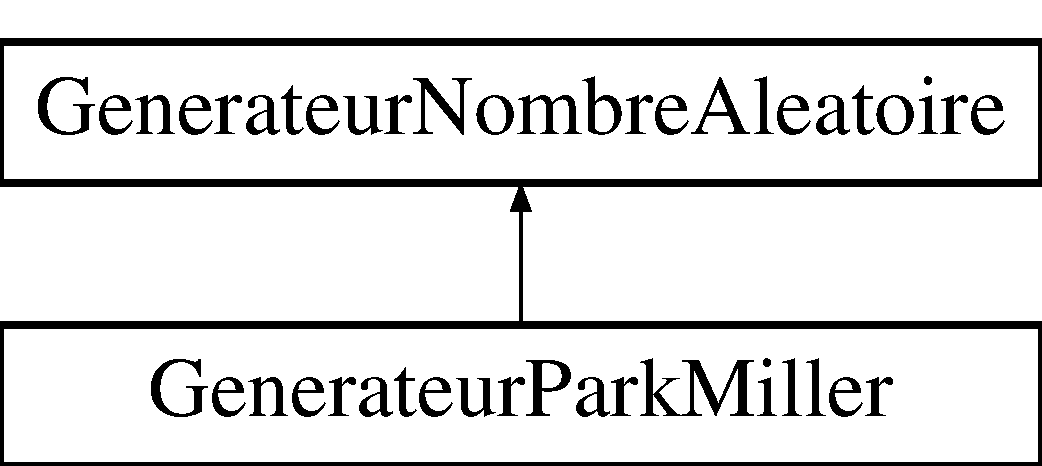
\includegraphics[height=2.000000cm]{classGenerateurParkMiller}
\end{center}
\end{figure}
\subsection*{Public Member Functions}
\begin{DoxyCompactItemize}
\item 
\hyperlink{classGenerateurParkMiller_a2fec69afe653b06bbea83ec62fbc5182}{Generateur\-Park\-Miller} ()
\item 
\hyperlink{classGenerateurParkMiller_ad71ea766644eb16e8ea11266ab989896}{Generateur\-Park\-Miller} (int dim)
\item 
\hyperlink{classGenerateurParkMiller_a70ceea9c05917df31cfa441e4b1ec076}{Generateur\-Park\-Miller} (const \hyperlink{classGenerateurParkMiller}{Generateur\-Park\-Miller} \&Gen)
\item 
\hyperlink{classGenerateurParkMiller}{Generateur\-Park\-Miller} $\ast$ \hyperlink{classGenerateurParkMiller_a84bd4dac445c2497e524ccc53a0333ac}{Clone} ()
\item 
\hyperlink{classGenerateurParkMiller_a6268a6b87c5dbc9652faa4b904cb82b5}{$\sim$\-Generateur\-Park\-Miller} ()
\item 
\hyperlink{classGenerateurParkMiller}{Generateur\-Park\-Miller} \hyperlink{classGenerateurParkMiller_ac7a10503745ddd060ef9c50d8dfaed79}{operator=} (const \hyperlink{classGenerateurParkMiller}{Generateur\-Park\-Miller} \&Gen)
\item 
int \hyperlink{classGenerateurParkMiller_a612cd197d36ff3fc2d8bef208f2ce5af}{get\-Dim} ()
\item 
void \hyperlink{classGenerateurParkMiller_ab011b6768425cf54d479ae82d188feb2}{set\-\_\-seed} (int seed)
\item 
int \hyperlink{classGenerateurParkMiller_a1b46d0c00bf5168e80b5f55f69ccdddb}{get\-\_\-seed} ()
\item 
void \hyperlink{classGenerateurParkMiller_a1c9cd0cd2a9ead72a3f20a83f25b7a67}{reset\-\_\-seed} ()
\item 
\hyperlink{classDvector}{Dvector} \hyperlink{classGenerateurParkMiller_a0bdd0f3185e1ee49f5d722f1dea59e2d}{gen\-Rand} ()
\end{DoxyCompactItemize}


\subsection{Constructor \& Destructor Documentation}
\hypertarget{classGenerateurParkMiller_a2fec69afe653b06bbea83ec62fbc5182}{\index{Generateur\-Park\-Miller@{Generateur\-Park\-Miller}!Generateur\-Park\-Miller@{Generateur\-Park\-Miller}}
\index{Generateur\-Park\-Miller@{Generateur\-Park\-Miller}!GenerateurParkMiller@{Generateur\-Park\-Miller}}
\subsubsection[{Generateur\-Park\-Miller}]{\setlength{\rightskip}{0pt plus 5cm}Generateur\-Park\-Miller\-::\-Generateur\-Park\-Miller (
\begin{DoxyParamCaption}
{}
\end{DoxyParamCaption}
)}}\label{classGenerateurParkMiller_a2fec69afe653b06bbea83ec62fbc5182}
\hypertarget{classGenerateurParkMiller_ad71ea766644eb16e8ea11266ab989896}{\index{Generateur\-Park\-Miller@{Generateur\-Park\-Miller}!Generateur\-Park\-Miller@{Generateur\-Park\-Miller}}
\index{Generateur\-Park\-Miller@{Generateur\-Park\-Miller}!GenerateurParkMiller@{Generateur\-Park\-Miller}}
\subsubsection[{Generateur\-Park\-Miller}]{\setlength{\rightskip}{0pt plus 5cm}Generateur\-Park\-Miller\-::\-Generateur\-Park\-Miller (
\begin{DoxyParamCaption}
\item[{int}]{dim}
\end{DoxyParamCaption}
)}}\label{classGenerateurParkMiller_ad71ea766644eb16e8ea11266ab989896}
\hypertarget{classGenerateurParkMiller_a70ceea9c05917df31cfa441e4b1ec076}{\index{Generateur\-Park\-Miller@{Generateur\-Park\-Miller}!Generateur\-Park\-Miller@{Generateur\-Park\-Miller}}
\index{Generateur\-Park\-Miller@{Generateur\-Park\-Miller}!GenerateurParkMiller@{Generateur\-Park\-Miller}}
\subsubsection[{Generateur\-Park\-Miller}]{\setlength{\rightskip}{0pt plus 5cm}Generateur\-Park\-Miller\-::\-Generateur\-Park\-Miller (
\begin{DoxyParamCaption}
\item[{const {\bf Generateur\-Park\-Miller} \&}]{Gen}
\end{DoxyParamCaption}
)}}\label{classGenerateurParkMiller_a70ceea9c05917df31cfa441e4b1ec076}
\hypertarget{classGenerateurParkMiller_a6268a6b87c5dbc9652faa4b904cb82b5}{\index{Generateur\-Park\-Miller@{Generateur\-Park\-Miller}!$\sim$\-Generateur\-Park\-Miller@{$\sim$\-Generateur\-Park\-Miller}}
\index{$\sim$\-Generateur\-Park\-Miller@{$\sim$\-Generateur\-Park\-Miller}!GenerateurParkMiller@{Generateur\-Park\-Miller}}
\subsubsection[{$\sim$\-Generateur\-Park\-Miller}]{\setlength{\rightskip}{0pt plus 5cm}Generateur\-Park\-Miller\-::$\sim$\-Generateur\-Park\-Miller (
\begin{DoxyParamCaption}
{}
\end{DoxyParamCaption}
)}}\label{classGenerateurParkMiller_a6268a6b87c5dbc9652faa4b904cb82b5}


\subsection{Member Function Documentation}
\hypertarget{classGenerateurParkMiller_a84bd4dac445c2497e524ccc53a0333ac}{\index{Generateur\-Park\-Miller@{Generateur\-Park\-Miller}!Clone@{Clone}}
\index{Clone@{Clone}!GenerateurParkMiller@{Generateur\-Park\-Miller}}
\subsubsection[{Clone}]{\setlength{\rightskip}{0pt plus 5cm}{\bf Generateur\-Park\-Miller} $\ast$ Generateur\-Park\-Miller\-::\-Clone (
\begin{DoxyParamCaption}
{}
\end{DoxyParamCaption}
)}}\label{classGenerateurParkMiller_a84bd4dac445c2497e524ccc53a0333ac}
\hypertarget{classGenerateurParkMiller_a0bdd0f3185e1ee49f5d722f1dea59e2d}{\index{Generateur\-Park\-Miller@{Generateur\-Park\-Miller}!gen\-Rand@{gen\-Rand}}
\index{gen\-Rand@{gen\-Rand}!GenerateurParkMiller@{Generateur\-Park\-Miller}}
\subsubsection[{gen\-Rand}]{\setlength{\rightskip}{0pt plus 5cm}{\bf Dvector} Generateur\-Park\-Miller\-::gen\-Rand (
\begin{DoxyParamCaption}
{}
\end{DoxyParamCaption}
)}}\label{classGenerateurParkMiller_a0bdd0f3185e1ee49f5d722f1dea59e2d}
\hypertarget{classGenerateurParkMiller_a1b46d0c00bf5168e80b5f55f69ccdddb}{\index{Generateur\-Park\-Miller@{Generateur\-Park\-Miller}!get\-\_\-seed@{get\-\_\-seed}}
\index{get\-\_\-seed@{get\-\_\-seed}!GenerateurParkMiller@{Generateur\-Park\-Miller}}
\subsubsection[{get\-\_\-seed}]{\setlength{\rightskip}{0pt plus 5cm}int Generateur\-Park\-Miller\-::get\-\_\-seed (
\begin{DoxyParamCaption}
{}
\end{DoxyParamCaption}
)}}\label{classGenerateurParkMiller_a1b46d0c00bf5168e80b5f55f69ccdddb}
\hypertarget{classGenerateurParkMiller_a612cd197d36ff3fc2d8bef208f2ce5af}{\index{Generateur\-Park\-Miller@{Generateur\-Park\-Miller}!get\-Dim@{get\-Dim}}
\index{get\-Dim@{get\-Dim}!GenerateurParkMiller@{Generateur\-Park\-Miller}}
\subsubsection[{get\-Dim}]{\setlength{\rightskip}{0pt plus 5cm}int Generateur\-Park\-Miller\-::get\-Dim (
\begin{DoxyParamCaption}
{}
\end{DoxyParamCaption}
)\hspace{0.3cm}{\ttfamily [inline]}}}\label{classGenerateurParkMiller_a612cd197d36ff3fc2d8bef208f2ce5af}
\hypertarget{classGenerateurParkMiller_ac7a10503745ddd060ef9c50d8dfaed79}{\index{Generateur\-Park\-Miller@{Generateur\-Park\-Miller}!operator=@{operator=}}
\index{operator=@{operator=}!GenerateurParkMiller@{Generateur\-Park\-Miller}}
\subsubsection[{operator=}]{\setlength{\rightskip}{0pt plus 5cm}{\bf Generateur\-Park\-Miller} Generateur\-Park\-Miller\-::operator= (
\begin{DoxyParamCaption}
\item[{const {\bf Generateur\-Park\-Miller} \&}]{Gen}
\end{DoxyParamCaption}
)}}\label{classGenerateurParkMiller_ac7a10503745ddd060ef9c50d8dfaed79}
\hypertarget{classGenerateurParkMiller_a1c9cd0cd2a9ead72a3f20a83f25b7a67}{\index{Generateur\-Park\-Miller@{Generateur\-Park\-Miller}!reset\-\_\-seed@{reset\-\_\-seed}}
\index{reset\-\_\-seed@{reset\-\_\-seed}!GenerateurParkMiller@{Generateur\-Park\-Miller}}
\subsubsection[{reset\-\_\-seed}]{\setlength{\rightskip}{0pt plus 5cm}void Generateur\-Park\-Miller\-::reset\-\_\-seed (
\begin{DoxyParamCaption}
{}
\end{DoxyParamCaption}
)}}\label{classGenerateurParkMiller_a1c9cd0cd2a9ead72a3f20a83f25b7a67}
\hypertarget{classGenerateurParkMiller_ab011b6768425cf54d479ae82d188feb2}{\index{Generateur\-Park\-Miller@{Generateur\-Park\-Miller}!set\-\_\-seed@{set\-\_\-seed}}
\index{set\-\_\-seed@{set\-\_\-seed}!GenerateurParkMiller@{Generateur\-Park\-Miller}}
\subsubsection[{set\-\_\-seed}]{\setlength{\rightskip}{0pt plus 5cm}void Generateur\-Park\-Miller\-::set\-\_\-seed (
\begin{DoxyParamCaption}
\item[{int}]{seed}
\end{DoxyParamCaption}
)}}\label{classGenerateurParkMiller_ab011b6768425cf54d479ae82d188feb2}


The documentation for this class was generated from the following files\-:\begin{DoxyCompactItemize}
\item 
src/\hyperlink{GenerateurParkMiller_8h}{Generateur\-Park\-Miller.\-h}\item 
src/\hyperlink{GenerateurParkMiller_8cpp}{Generateur\-Park\-Miller.\-cpp}\end{DoxyCompactItemize}

\hypertarget{classParkMiller}{\section{Park\-Miller Class Reference}
\label{classParkMiller}\index{Park\-Miller@{Park\-Miller}}
}


{\ttfamily \#include $<$Park\-Miller.\-h$>$}

\subsection*{Public Member Functions}
\begin{DoxyCompactItemize}
\item 
\hyperlink{classParkMiller_aa3ff1e9965841612a8b68a83b3553723}{Park\-Miller} ()
\item 
\hyperlink{classParkMiller_a31033c0208b9778481039065e3c69b4d}{Park\-Miller} (const \hyperlink{classParkMiller}{Park\-Miller} \&P)
\item 
\hyperlink{classParkMiller_a8d36ad067775b28836561f9ec844f058}{$\sim$\-Park\-Miller} ()
\item 
\hyperlink{classParkMiller}{Park\-Miller} \hyperlink{classParkMiller_a7ba3edad2f29deededee38106a3c029a}{operator=} (const \hyperlink{classParkMiller}{Park\-Miller} \&P)
\item 
int \hyperlink{classParkMiller_aad562b2b5b91bf67c78027e91ab55d2d}{get\-Seed} ()
\item 
void \hyperlink{classParkMiller_a2c878610bd1f0e06a8c91b98d63f1a40}{set\-Seed} (int \hyperlink{classParkMiller_a425ab2a4cf6f25d7749285286b3504d7}{seed})
\item 
double \hyperlink{classParkMiller_afd66989754d5fff50da023ca899dc68f}{gen\-Random} ()
\end{DoxyCompactItemize}
\subsection*{Protected Attributes}
\begin{DoxyCompactItemize}
\item 
int \hyperlink{classParkMiller_a425ab2a4cf6f25d7749285286b3504d7}{seed}
\end{DoxyCompactItemize}


\subsection{Constructor \& Destructor Documentation}
\hypertarget{classParkMiller_aa3ff1e9965841612a8b68a83b3553723}{\index{Park\-Miller@{Park\-Miller}!Park\-Miller@{Park\-Miller}}
\index{Park\-Miller@{Park\-Miller}!ParkMiller@{Park\-Miller}}
\subsubsection[{Park\-Miller}]{\setlength{\rightskip}{0pt plus 5cm}Park\-Miller\-::\-Park\-Miller (
\begin{DoxyParamCaption}
{}
\end{DoxyParamCaption}
)}}\label{classParkMiller_aa3ff1e9965841612a8b68a83b3553723}
\hypertarget{classParkMiller_a31033c0208b9778481039065e3c69b4d}{\index{Park\-Miller@{Park\-Miller}!Park\-Miller@{Park\-Miller}}
\index{Park\-Miller@{Park\-Miller}!ParkMiller@{Park\-Miller}}
\subsubsection[{Park\-Miller}]{\setlength{\rightskip}{0pt plus 5cm}Park\-Miller\-::\-Park\-Miller (
\begin{DoxyParamCaption}
\item[{const {\bf Park\-Miller} \&}]{P}
\end{DoxyParamCaption}
)}}\label{classParkMiller_a31033c0208b9778481039065e3c69b4d}
\hypertarget{classParkMiller_a8d36ad067775b28836561f9ec844f058}{\index{Park\-Miller@{Park\-Miller}!$\sim$\-Park\-Miller@{$\sim$\-Park\-Miller}}
\index{$\sim$\-Park\-Miller@{$\sim$\-Park\-Miller}!ParkMiller@{Park\-Miller}}
\subsubsection[{$\sim$\-Park\-Miller}]{\setlength{\rightskip}{0pt plus 5cm}Park\-Miller\-::$\sim$\-Park\-Miller (
\begin{DoxyParamCaption}
{}
\end{DoxyParamCaption}
)}}\label{classParkMiller_a8d36ad067775b28836561f9ec844f058}


\subsection{Member Function Documentation}
\hypertarget{classParkMiller_afd66989754d5fff50da023ca899dc68f}{\index{Park\-Miller@{Park\-Miller}!gen\-Random@{gen\-Random}}
\index{gen\-Random@{gen\-Random}!ParkMiller@{Park\-Miller}}
\subsubsection[{gen\-Random}]{\setlength{\rightskip}{0pt plus 5cm}double Park\-Miller\-::gen\-Random (
\begin{DoxyParamCaption}
{}
\end{DoxyParamCaption}
)}}\label{classParkMiller_afd66989754d5fff50da023ca899dc68f}
\hypertarget{classParkMiller_aad562b2b5b91bf67c78027e91ab55d2d}{\index{Park\-Miller@{Park\-Miller}!get\-Seed@{get\-Seed}}
\index{get\-Seed@{get\-Seed}!ParkMiller@{Park\-Miller}}
\subsubsection[{get\-Seed}]{\setlength{\rightskip}{0pt plus 5cm}int Park\-Miller\-::get\-Seed (
\begin{DoxyParamCaption}
{}
\end{DoxyParamCaption}
)\hspace{0.3cm}{\ttfamily [inline]}}}\label{classParkMiller_aad562b2b5b91bf67c78027e91ab55d2d}
\hypertarget{classParkMiller_a7ba3edad2f29deededee38106a3c029a}{\index{Park\-Miller@{Park\-Miller}!operator=@{operator=}}
\index{operator=@{operator=}!ParkMiller@{Park\-Miller}}
\subsubsection[{operator=}]{\setlength{\rightskip}{0pt plus 5cm}{\bf Park\-Miller} Park\-Miller\-::operator= (
\begin{DoxyParamCaption}
\item[{const {\bf Park\-Miller} \&}]{P}
\end{DoxyParamCaption}
)}}\label{classParkMiller_a7ba3edad2f29deededee38106a3c029a}
\hypertarget{classParkMiller_a2c878610bd1f0e06a8c91b98d63f1a40}{\index{Park\-Miller@{Park\-Miller}!set\-Seed@{set\-Seed}}
\index{set\-Seed@{set\-Seed}!ParkMiller@{Park\-Miller}}
\subsubsection[{set\-Seed}]{\setlength{\rightskip}{0pt plus 5cm}void Park\-Miller\-::set\-Seed (
\begin{DoxyParamCaption}
\item[{int}]{seed}
\end{DoxyParamCaption}
)\hspace{0.3cm}{\ttfamily [inline]}}}\label{classParkMiller_a2c878610bd1f0e06a8c91b98d63f1a40}


\subsection{Member Data Documentation}
\hypertarget{classParkMiller_a425ab2a4cf6f25d7749285286b3504d7}{\index{Park\-Miller@{Park\-Miller}!seed@{seed}}
\index{seed@{seed}!ParkMiller@{Park\-Miller}}
\subsubsection[{seed}]{\setlength{\rightskip}{0pt plus 5cm}int Park\-Miller\-::seed\hspace{0.3cm}{\ttfamily [protected]}}}\label{classParkMiller_a425ab2a4cf6f25d7749285286b3504d7}


The documentation for this class was generated from the following files\-:\begin{DoxyCompactItemize}
\item 
src/\hyperlink{ParkMiller_8h}{Park\-Miller.\-h}\item 
src/\hyperlink{ParkMiller_8cpp}{Park\-Miller.\-cpp}\end{DoxyCompactItemize}

\chapter{File Documentation}
\hypertarget{Dvector_8cpp}{\section{src/\-Dvector.cpp File Reference}
\label{Dvector_8cpp}\index{src/\-Dvector.\-cpp@{src/\-Dvector.\-cpp}}
}
{\ttfamily \#include \char`\"{}Dvector.\-h\char`\"{}}\\*
{\ttfamily \#include $<$stdio.\-h$>$}\\*
{\ttfamily \#include $<$stdlib.\-h$>$}\\*
{\ttfamily \#include $<$time.\-h$>$}\\*
{\ttfamily \#include $<$fstream$>$}\\*
{\ttfamily \#include $<$string$>$}\\*
{\ttfamily \#include $<$cstring$>$}\\*
\subsection*{Functions}
\begin{DoxyCompactItemize}
\item 
\hyperlink{classDvector}{Dvector} \hyperlink{Dvector_8cpp_adc04cf82aee079aca57cf20806737afe}{operator+} (const \hyperlink{classDvector}{Dvector} \&n, const \hyperlink{classDvector}{Dvector} \&v)
\item 
\hyperlink{classDvector}{Dvector} \hyperlink{Dvector_8cpp_a73a2612ede73afd8f5e94fa2ae0d6aa4}{operator-\/} (const \hyperlink{classDvector}{Dvector} \&n, const \hyperlink{classDvector}{Dvector} \&v)
\item 
bool \hyperlink{Dvector_8cpp_a78765ce7576547b645ccc54e0b22e7bf}{operator==} (const \hyperlink{classDvector}{Dvector} \&n, const \hyperlink{classDvector}{Dvector} \&v)
\end{DoxyCompactItemize}


\subsection{Function Documentation}
\hypertarget{Dvector_8cpp_adc04cf82aee079aca57cf20806737afe}{\index{Dvector.\-cpp@{Dvector.\-cpp}!operator+@{operator+}}
\index{operator+@{operator+}!Dvector.cpp@{Dvector.\-cpp}}
\subsubsection[{operator+}]{\setlength{\rightskip}{0pt plus 5cm}{\bf Dvector} operator+ (
\begin{DoxyParamCaption}
\item[{const {\bf Dvector} \&}]{n, }
\item[{const {\bf Dvector} \&}]{v}
\end{DoxyParamCaption}
)}}\label{Dvector_8cpp_adc04cf82aee079aca57cf20806737afe}
\hypertarget{Dvector_8cpp_a73a2612ede73afd8f5e94fa2ae0d6aa4}{\index{Dvector.\-cpp@{Dvector.\-cpp}!operator-\/@{operator-\/}}
\index{operator-\/@{operator-\/}!Dvector.cpp@{Dvector.\-cpp}}
\subsubsection[{operator-\/}]{\setlength{\rightskip}{0pt plus 5cm}{\bf Dvector} operator-\/ (
\begin{DoxyParamCaption}
\item[{const {\bf Dvector} \&}]{n, }
\item[{const {\bf Dvector} \&}]{v}
\end{DoxyParamCaption}
)}}\label{Dvector_8cpp_a73a2612ede73afd8f5e94fa2ae0d6aa4}
\hypertarget{Dvector_8cpp_a78765ce7576547b645ccc54e0b22e7bf}{\index{Dvector.\-cpp@{Dvector.\-cpp}!operator==@{operator==}}
\index{operator==@{operator==}!Dvector.cpp@{Dvector.\-cpp}}
\subsubsection[{operator==}]{\setlength{\rightskip}{0pt plus 5cm}bool operator== (
\begin{DoxyParamCaption}
\item[{const {\bf Dvector} \&}]{n, }
\item[{const {\bf Dvector} \&}]{v}
\end{DoxyParamCaption}
)}}\label{Dvector_8cpp_a78765ce7576547b645ccc54e0b22e7bf}

\hypertarget{Dvector_8h}{\section{src/\-Dvector.h File Reference}
\label{Dvector_8h}\index{src/\-Dvector.\-h@{src/\-Dvector.\-h}}
}


Classe implémentant des tableaux dynamiques et les opérations allant avec.  


{\ttfamily \#include $<$iostream$>$}\\*
\subsection*{Classes}
\begin{DoxyCompactItemize}
\item 
class \hyperlink{classDvector}{Dvector}
\end{DoxyCompactItemize}


\subsection{Detailed Description}
Classe implémentant des tableaux dynamiques et les opérations allant avec. \begin{DoxyAuthor}{Author}
morel2-\/malafost 
\end{DoxyAuthor}

\hypertarget{GenerateurNombreAleatoire_8cpp}{\section{src/\-Generateur\-Nombre\-Aleatoire.cpp File Reference}
\label{GenerateurNombreAleatoire_8cpp}\index{src/\-Generateur\-Nombre\-Aleatoire.\-cpp@{src/\-Generateur\-Nombre\-Aleatoire.\-cpp}}
}
{\ttfamily \#include \char`\"{}Generateur\-Nombre\-Aleatoire.\-h\char`\"{}}\\*

\hypertarget{GenerateurNombreAleatoire_8h}{\section{src/\-Generateur\-Nombre\-Aleatoire.h File Reference}
\label{GenerateurNombreAleatoire_8h}\index{src/\-Generateur\-Nombre\-Aleatoire.\-h@{src/\-Generateur\-Nombre\-Aleatoire.\-h}}
}
{\ttfamily \#include \char`\"{}Dvector.\-h\char`\"{}}\\*
\subsection*{Classes}
\begin{DoxyCompactItemize}
\item 
class \hyperlink{classGenerateurNombreAleatoire}{Generateur\-Nombre\-Aleatoire}
\end{DoxyCompactItemize}

\hypertarget{GenerateurParkMiller_8cpp}{\section{src/\-Generateur\-Park\-Miller.cpp File Reference}
\label{GenerateurParkMiller_8cpp}\index{src/\-Generateur\-Park\-Miller.\-cpp@{src/\-Generateur\-Park\-Miller.\-cpp}}
}
{\ttfamily \#include \char`\"{}Generateur\-Park\-Miller.\-h\char`\"{}}\\*

\hypertarget{GenerateurParkMiller_8h}{\section{src/\-Generateur\-Park\-Miller.h File Reference}
\label{GenerateurParkMiller_8h}\index{src/\-Generateur\-Park\-Miller.\-h@{src/\-Generateur\-Park\-Miller.\-h}}
}
{\ttfamily \#include \char`\"{}Generateur\-Nombre\-Aleatoire.\-h\char`\"{}}\\*
{\ttfamily \#include \char`\"{}Park\-Miller.\-h\char`\"{}}\\*
\subsection*{Classes}
\begin{DoxyCompactItemize}
\item 
class \hyperlink{classGenerateurParkMiller}{Generateur\-Park\-Miller}
\end{DoxyCompactItemize}

\hypertarget{gentest_8cpp}{\section{src/gentest.cpp File Reference}
\label{gentest_8cpp}\index{src/gentest.\-cpp@{src/gentest.\-cpp}}
}
{\ttfamily \#include $<$iostream$>$}\\*
{\ttfamily \#include $<$string$>$}\\*
{\ttfamily \#include $<$sstream$>$}\\*
{\ttfamily \#include $<$assert.\-h$>$}\\*
{\ttfamily \#include \char`\"{}Generateur\-Park\-Miller.\-h\char`\"{}}\\*
\subsection*{Functions}
\begin{DoxyCompactItemize}
\item 
int \hyperlink{gentest_8cpp_ae66f6b31b5ad750f1fe042a706a4e3d4}{main} ()
\end{DoxyCompactItemize}


\subsection{Function Documentation}
\hypertarget{gentest_8cpp_ae66f6b31b5ad750f1fe042a706a4e3d4}{\index{gentest.\-cpp@{gentest.\-cpp}!main@{main}}
\index{main@{main}!gentest.cpp@{gentest.\-cpp}}
\subsubsection[{main}]{\setlength{\rightskip}{0pt plus 5cm}int main (
\begin{DoxyParamCaption}
{}
\end{DoxyParamCaption}
)}}\label{gentest_8cpp_ae66f6b31b5ad750f1fe042a706a4e3d4}

\hypertarget{main_8cpp}{\section{src/main.cpp File Reference}
\label{main_8cpp}\index{src/main.\-cpp@{src/main.\-cpp}}
}
{\ttfamily \#include $<$iostream$>$}\\*
{\ttfamily \#include $<$string$>$}\\*
{\ttfamily \#include $<$sstream$>$}\\*
{\ttfamily \#include $<$assert.\-h$>$}\\*
{\ttfamily \#include \char`\"{}Dvector.\-h\char`\"{}}\\*
\subsection*{Functions}
\begin{DoxyCompactItemize}
\item 
int \hyperlink{main_8cpp_ae66f6b31b5ad750f1fe042a706a4e3d4}{main} ()
\end{DoxyCompactItemize}


\subsection{Function Documentation}
\hypertarget{main_8cpp_ae66f6b31b5ad750f1fe042a706a4e3d4}{\index{main.\-cpp@{main.\-cpp}!main@{main}}
\index{main@{main}!main.cpp@{main.\-cpp}}
\subsubsection[{main}]{\setlength{\rightskip}{0pt plus 5cm}int main (
\begin{DoxyParamCaption}
{}
\end{DoxyParamCaption}
)}}\label{main_8cpp_ae66f6b31b5ad750f1fe042a706a4e3d4}

\hypertarget{ParkMiller_8cpp}{\section{src/\-Park\-Miller.cpp File Reference}
\label{ParkMiller_8cpp}\index{src/\-Park\-Miller.\-cpp@{src/\-Park\-Miller.\-cpp}}
}
{\ttfamily \#include $<$iostream$>$}\\*
{\ttfamily \#include $<$math.\-h$>$}\\*
{\ttfamily \#include $<$stdlib.\-h$>$}\\*
{\ttfamily \#include \char`\"{}Park\-Miller.\-h\char`\"{}}\\*

\hypertarget{ParkMiller_8h}{\section{src/\-Park\-Miller.h File Reference}
\label{ParkMiller_8h}\index{src/\-Park\-Miller.\-h@{src/\-Park\-Miller.\-h}}
}
\subsection*{Classes}
\begin{DoxyCompactItemize}
\item 
class \hyperlink{classParkMiller}{Park\-Miller}
\end{DoxyCompactItemize}

%--- End generated contents ---

% Index
\newpage
\phantomsection
\addcontentsline{toc}{part}{Index}
\printindex

\end{document}
